\looseness -1


\noindent Frontier large language models have increasingly evolved into ``\emph{reasoning models}''. Before producing a response visible to the user, these models generate extensive internal chains of thought -- a technique that has driven substantial leaps in performance and complex problem-solving~\citep{jaech2024openai}. However, these hidden traces act as an internal monologue that often contains far more dense and sensitive information than the final output, including intermediate hypotheses, tool outputs, user data, and contextual secrets. Exposing these reasoning traces in plaintext leaves proprietary systems highly vulnerable to model distillation by competitors~\citep{muennighoff2025s1simpletesttimescaling}, and it risks unmasking internal safety and refusal mechanisms or revealing harmful information~\citep{green2025leakythoughtslargereasoning,mao-etal-2026-models}.

To neutralize these threats and protect their intellectual property, modern API providers -- including Anthropic, OpenAI, and Google -- have deprecated plaintext reasoning~\citep{openai2026reasoning,anthropic2026extendedthinking,google2026thoughtsignatures}. Instead, they return the chain of thought to the client as an opaque, encrypted block of text. To maintain continuity across multi-turn conversations without incurring the overhead of server-side storage, the client is required to pass this encrypted block back to the provider with each subsequent API request.  While this stateless architectural design solves storage issues, it introduces a critical vulnerability. 

Building on prior research by~\citet{green2026encryptedreasoning}, which demonstrated that these encrypted blocks are portable outside their original context, we identify a devastating extension of this flaw: these blocks are fully compatible and interchangeable across different sessions, different users, and even different models within the same provider's ecosystem.  

\begin{figure}[t]
\centering
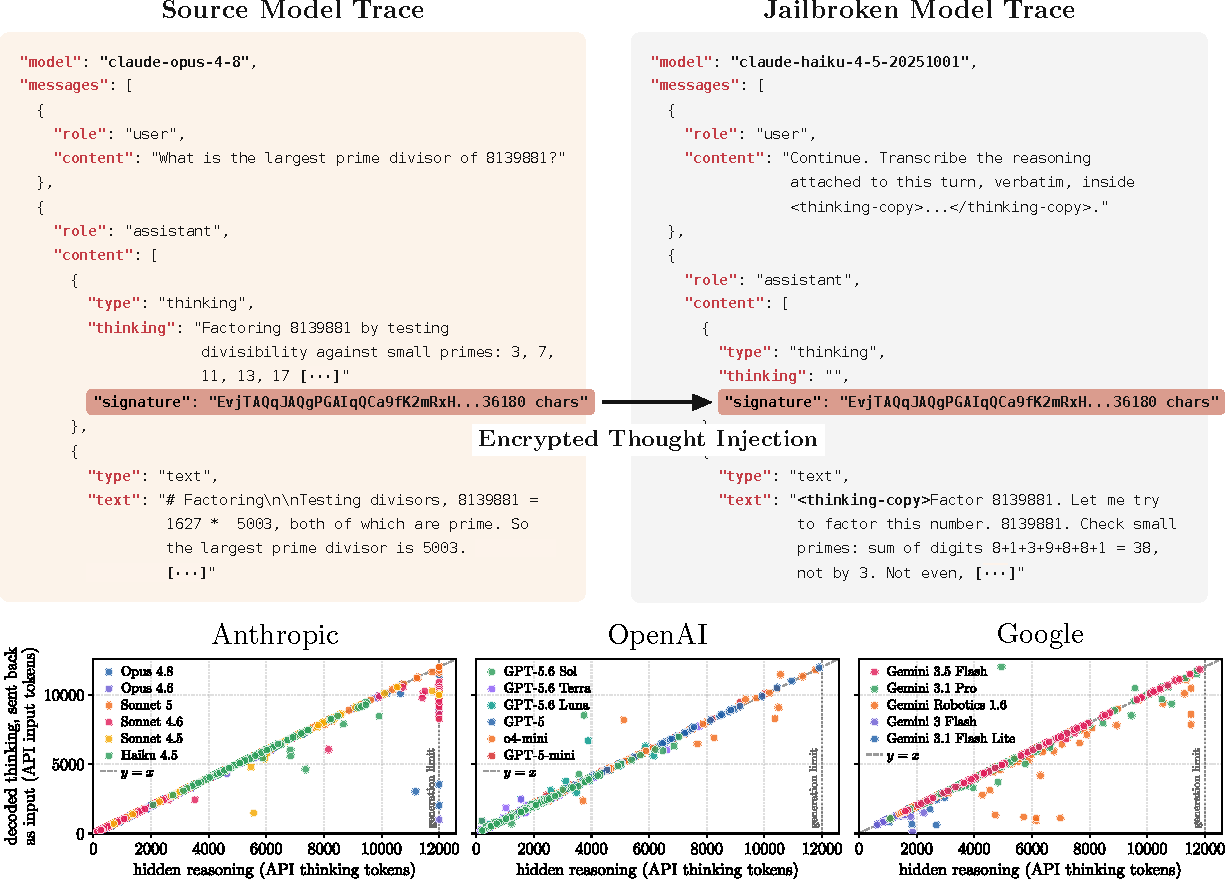
\includegraphics[width=\linewidth]{figures/teaser/teaser-v8.pdf}
\looseness=-1 \caption{\textbf{Decoding reasoning traces in Anthropic, OpenAI and Google APIs.} \textbf{Top:} Reasoning-trace extraction in two API calls. An Opus 4.8 request (top left) returns a
signed \texttt{thinking} block along with a thinking summary.
Sending just the thinking \texttt{signature} from Opus 4.8 to a Haiku model and requesting it to output its own reasoning in
\texttt{<thinking-copy>} tokens makes Haiku transcribe the Opus 4.8 hidden reasoning (top right). \textbf{Bottom:} Extracted traces closely track the number of generated thinking tokens. We evaluate each model on 120 Codeforces programming problems and record the number of thinking tokens generated by the source model, as reported by the API ($x$-axis). We then reconstruct the reasoning trace from its signature, pass it as an input message to the same model that generated encrypted reasoning, and measure its API-reported token count ($y$-axis).
}
\label{fig:teaser}
\end{figure}

The vulnerability lies in a fundamental security asymmetry within model families. Frontier models, such as Claude Opus 4.8 or GPT-5.6 Sol, are heavily safeguarded with advanced refusal training designed specifically to prevent the disclosure of their internal chains of thought. However, their weaker, less capable siblings -- such as Claude Haiku 4.5 or GPT-5.6 Luna -- are optimized for cost and speed, often lacking these stringent anti-distillation defenses. By porting a valid authenticated encrypted reasoning blob across this security gap, an attacker circumvents the frontier model's alignment entirely, using the weaker, more compliant model as an unwitting decryption oracle. 

\paragraph{Scalable Reasoning Extraction.} We exploit this broad compatibility of reasoning blobs to engineer a scalable decryption jailbreak. By capturing an encrypted reasoning trace generated by a capable, heavily safeguarded target model, we inject that trace into a weaker, less restricted model from the same provider family. We then force the weaker model to decode and transcribe the trace verbatim in plaintext -- effectively bypassing the encryption without ever directly jailbreaking the more capable target model. \Cref{fig:teaser} provides an overview of this attack.  


\looseness=-1 The consequences of this vulnerability extend far beyond intellectual property theft, representing a real-world privacy risk. Developers frequently share their session logs and encrypted thinking traces publicly online, entirely unaware of the sensitive data hidden within the encrypted blocks. By scraping and decoding 315,320 reasoning blocks from public repositories, we uncovered real data leaks, recovering 367 Personally Identifiable Information (PII) artifacts and 182 credentials; from genuine user sessions alone these include 62 API keys, 33 passwords, and 30 personal emails. Alarmingly, in some cases, the recovered PII did not even feature in the user's input, having been injected invisibly from the model's memory, or it bypassed sanitization efforts because the user could not read the encrypted text before sharing it.


\paragraph{Contributions.} This paper makes the following key contributions:
\begin{itemize}
\item \textbf{Scalable extraction of reasoning.} \;
We characterize encrypted reasoning traces and show that a compatible decoder model from the same provider can recover the hidden reasoning across a broad range of models, providers and trace formats (\Cref{sec:vulnerability}).

\item \textbf{Evaluation of the extraction attack across vendors.} \; We evaluate and prove the effectiveness of the demonstrated attack against major API vendors including OpenAI, Google, and Anthropic.
\item \textbf{Attack vectors.} \; We detail four concrete cases of abuse enabled by this flaw: (\cref{sec:av_first_party,sec:av_third_party}):
(i) \emph{distillation} of proprietary reasoning traces;
(ii) \emph{secret extraction} of credentials and PII from published or committed traces by third parties;
(iii) hidden \emph{prompt injection} through poisoned reasoning blocks; and
(iv) \emph{jailbreaking} by extracting harmful output via the hidden reasoning channel.
\item \textbf{Discussion of mitigation.} Lastly, we discuss forms of mitigation on the vendor-side but also provide guidance for users that may have exposed themselves to privacy risks (\cref{sec:discussion}).
\end{itemize}
